\documentclass{article}

\usepackage{enumitem}
\usepackage{amsmath}
\usepackage{amsfonts}
\usepackage[dvipsnames]{xcolor}
\usepackage{amssymb}
\usepackage[margin=0.5in]{geometry}
\usepackage[hidelinks, bookmarks=false]{hyperref}

\usepackage{tkz-berge}

\graphicspath{{.}{./img/}}

\let\oldemptyset\emptyset
\let\emptyset\varnothing
\let\oldepsilon\epsilon
\let\epsilon\varepsilon
\newcommand{\N}{\mathbb{N}}
\newcommand{\R}{\mathbb{R}}
\newcommand{\Q}{\mathbb{Q}}

\usepackage{environ}
\NewEnviron{centerframebox}{\begin{center}\fbox{\parbox{0.92\textwidth}{\BODY}}\end{center}}

\title{Combinatorial Optimization \\ Exercise Set 7 \\ Tuesday class}
\author{
  \AA{AAAAAAAAAA AAAAAAA}{6} \\
  \href{mailto:\AA{AAAAAAAAAAAAAAAAAAAA}{7}}{\AA{AAAAAAAAAAAAAAAAAAAA}{7}}
  \and
  Carola Ley \\
  \href{mailto:s6caleyy@uni-bonn.de}{s6caleyy@uni-bonn.de}
  \and
  Bailee Zacovic \\
  \href{mailto:s38bzaco@uni-bonn.de}{s38bzaco@uni-bonn.de}
}

\begin{document}
  \maketitle

  \setcounter{section}{7}
  \subsection{Metric edge connectivities}
  \begin{centerframebox}
    Let $\lambda_{ij},\; 1 \leq i, j \leq n$, be nonnegative numbers with $\lambda_{ij} = \lambda_{ji}$ and
    $\lambda_{ik} \geq \min\{\lambda_{ij},\, \lambda_{jk}\}$ for any three distinct indices $i,\, j,\, k \in \{1,\, \dots,\, n\}$.
    Show that there exists a graph $G$ with $V(G) = \{1,\, \dots,\, n\}$ and capacities $u: E(G) \to \R_+$ such
    that the local edge-connectivities are precisely the $\lambda_{ij}$.

    Hint: Consider a maximum weight spanning tree in $(K_n,\, c)$, where $c(\{i,\, j\}) := \lambda_{ij}$.
  \end{centerframebox}
  Let $\lambda_{ij},\; 1 \leq i, j \leq n$, be nonnegative numbers with $\lambda_{ij} = \lambda_{ji}$ and $\lambda_{ik} \geq \min\{\lambda_{ij},\, \lambda_{jk}\}$ for any three distinct indices $i,\, j,\, k \in \{1,\, \dots,\, n\}$. Fix a maximum weight spanning tree $T$ in $(K_n,c)$ where $c:E(K_n)\rightarrow \mathbb{R}_{\geq 0}$ is given by $c(\{i,j\})=\lambda_{ij}$ for all $1\leq i,j,\leq n.$ Let $M=\{e\in E(K_n):c(e)=0\}.$ We claim that $(G,u)=(T\setminus M,c)$ satisfies the claim. To this end, it suffices to check that the minimum capacity $i$-$j$ cut in $T\setminus M$ for any $i\neq j$ is given by $\lambda_{ij}.$

  Fix $i\neq j.$ Since $T$ is a tree, there is a unique $i$-$j$-path $P_{ij}$ on vertices $i=m_0, m_1,m_2,\dots,m_r=j,$ where the minimum capacity $i$-$j$ cut is given by $\min\{\lambda_{m_0m_1},\lambda_{m_2m_2},\dots,\lambda_{m_{r-1}m_r}\}.$ It is clear by hypothesis, $$\lambda_{ij} \geq \min\{\lambda_{m_0m_1},\lambda_{m_2m_2},\dots,\lambda_{m_{r-1}m_r}\}.$$ We argue that \begin{equation}\lambda_{ij} \leq \min\{\lambda_{m_0m_1},\lambda_{m_2m_2},\dots,\lambda_{m_{r-1}m_r}\}.\end{equation}
  When $|P_{ij}|=1$, this follows immediately. When $|P_{ij}|>1,$ suppose $\lambda_{ij} > \min\{\lambda_{m_0m_1},\lambda_{m_2m_2},\dots,\lambda_{m_{r-1}m_r}\}$. Since the minimum is achieved on $P_{ij},$ this amounts to saying $\lambda_{ij}>\lambda_{m_{\ell-1}m_{\ell}}$ for some $1\leq \ell\leq r.$ But then $T':=(T\setminus \{\ell-1,\ell\})\cup \{i,j\}$ would be a spanning tree with total weight $$\sum_{\{s,t\}\in E(T)}\lambda_{st}+(\lambda_{ij}-\lambda_{\ell-1\ell})>\sum_{\{s,t\}\in E(T)}\lambda_{st},$$contradicting that $T$ is a maximum weight spanning tree.
  From (1) it follows that $\lambda_{ij} = \min\{\lambda_{m_0m_1},\lambda_{m_2m_2},\dots,\lambda_{m_{r-1}m_r}\}$ does indeed give the local edge connectivity for all vertices. In particular, $\lambda_{ij}=0$ if and only if $P_{ij}$ in $T$ includes an edge $\{m_{\ell-1},m_{\ell}\}\in M$, which occurs if and only if $i$ and $j$ lie in different connected components of $T\setminus M.$ Hence the claim holds for $(T\setminus M,c).$ $\blacksquare$

  \subsection{Wrong spanning-tree polytope}
  \begin{centerframebox}
    For an undirected graph $G$, let $P_G$ denote the spanning-tree polytope of $G$ and

    \[ Q_{G} := \left\{
      x\in[0,1]^{E(G)}:
      \sum_{e\in E(G)} x_{e} = |V(G)|-1 \;,\;
      \sum_{e\in\delta(X)}x_{e} \geq 1
      \textrm{ for } \emptyset \neq X \subsetneq V(G) \right\}. \]

    Prove:
    \begin{enumerate}[label=(\roman*)]
      \item $P_G \subseteq Q_G$ for every graph $G$.
      \item There exists a graph $G$ with $P_G \neq Q_G$.
    \end{enumerate}

    The real spanning-tree polytope $P_G$ is:
    \[ P_{G} := \left\{
      x\in[0,1]^{E(G)}:
      \sum_{e\in E(G)} x_{e} = |V(G)|-1 \;,\;
      \sum_{e\in E(G[X])} x_{e} \leq |X|-1
      \textrm{ for } \emptyset \neq X \subsetneq V(G) \right\}. \]
    %
  \end{centerframebox}
  \subsubsection*{(i) $P_G \subseteq Q_G$ for every graph $G$.}
  We can derive the $\sum_{e\in\delta(X)}x_{e} \geq 1$ condition from its equivalent in the $P_G$ polytope with some simple algebra.
  Consider the two vertex sets: $X$ and its compliment $V(G) \setminus X$.
  Together with the cut $\delta(X)$ they will cover all the edges of $G$ exactly once,
  so we can combine the inequalities with the condition that the total amount of edges must be equal to $|V(G)|-1$:
  \[ \sum_{e\in E(G[X])} x_{e} \leq |X|-1 \qquad
     \sum_{e\in E(G[V(G) \setminus X])} x_{e} \leq |V(G)|-|X|-1 \]
  \[ \sum_{e\in\delta(X)}x_{e} = |V(G)|-1 - \sum_{e\in E(G[X])} x_{e} - \sum_{e\in E(G[V(G) \setminus X])} x_{e} \]
  \begin{align*}
     \sum_{e\in\delta(X)}x_{e} &\geq |V(G)|-1 - (|X|-1) - (|V(G)|-|X|-1)\\
    %  &\geq |V(G)|-1 - |X|+1 - |V(G)|+|X|+1 \\
     &\geq 1
  \end{align*}
  So we derived the condition for the $Q_G$ polytope from the $P_G$, so $P_G \subseteq Q_G$.
  $\blacksquare$

  \subsubsection*{(ii) There exists a graph $G$ with $P_G \neq Q_G$.}
  To find a counterexample, we can assume that there exists $\exists X' \subsetneq V(G) : \sum_{e\in E(G[X'])} x_{e} = |X'|$
  with the lowest possible value that excludes it from $P_G$, and see what will follow from this assumption.
  We can use the same $V(G) \setminus X$ trick here:
  \[ |V(G)| - 1 = \sum_{e\in E(G[X'])} x_{e} + \sum_{e\in E(G[V(G) \setminus X'])} x_{e} + \sum_{e\in\delta(X')}x_{e} \]
  \[ \sum_{e\in E(G[V(G) \setminus X'])} x_{e} = |V(G)| - 1 - \sum_{e\in E(G[X'])} x_{e} - \sum_{e\in\delta(X')}x_{e} \]
  \[ \sum_{e\in E(G[V(G) \setminus X'])} x_{e} \leq |V(G)| - 1 - |X'| - 1 \]
  \[ \sum_{e\in E(G[V(G) \setminus X'])} x_{e} \leq |V(G)| - |X'| - 2 \]
  This way we changed the cycle constraint for $V(G) \setminus X'$ form $|V(G)| - |X'| - 1$ to $|V(G)| - |X'| - 2$.

  Let's try constructing such a graph, with $\sum_{e\in E(G[X'])} x_{e} = |X'|$ and $\sum_{e\in E(G[V(G) \setminus X'])} x_{e} = |V(G) \setminus X'| - 2$:
  \begin{center}
    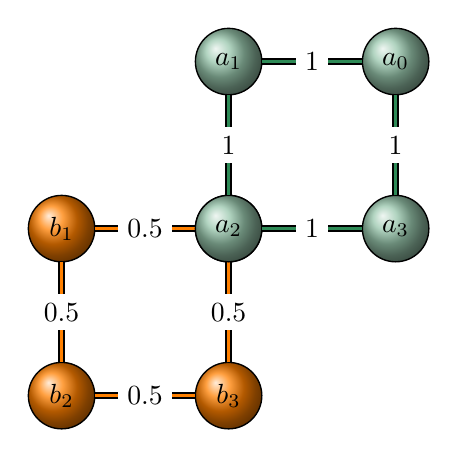
\begin{tikzpicture}
      \SetVertexMath
      \GraphInit[vstyle=Shade]
      \grCycle[prefix=b,rotation=45,RA=1.5]{4}
      \Edges[label=$0.5$](b1,b2,b3,b0,b1)
      \begin{scope}[xshift=2.1213cm,yshift=2.1213cm]
        \SetGraphShadeColor{SeaGreen!50}{black}{SeaGreen}
        \grCycle[prefix=a,rotation=45,RA=1.5]{4}
        \Edges[label=$1$](a1,a2,a3,a0,a1)
      \end{scope}
    \end{tikzpicture}
  \end{center}
  The vertices in $X'$ are represented by $a_0,\dots,a_3$ and the vertices in $V(G) \setminus X'$ by $b_1,\dots,b_3$.
  We can see that this particular incidence vector $x$, represented by the edge labels, is not in $P_G$,
  because $\sum_{e\in E(G[X'])} x_{e} = |X'| = 4$.
  But the sum of all edges $ \sum_{e\in E(G)} x_{e} = 0.5 \cdot 4 + 4 = 6 = |V(G)|-1 = 7-1$
  and the cut condition also holds (the graph is connected and every vertex has its edges sum to at least $1$),
  so $x \in Q_G$ and we found our counterexample.

  \subsection{$b$-matching criterion}
  \begin{centerframebox}
    Let $G$ be a graph, $u: E(G) \to \N \cup \{\infty\}$ and $b : V (G) \to \N$.
    Show that $(G, u)$ has a perfect $b$-matching if and only if for any two disjoint subsets
    $X,\, Y \subseteq V (G)$ the number of connected components $C$ in $G - X - Y$ for which
    $\sum_{c\in V(C)}b(c) + \sum_{e\in E_G(V(C),Y)}u(e)$
    is odd does not exceed
    \[ \sum_{v\in X}b(v)+\sum_{y\in Y}\left(\sum_{e\in\delta(y)}u(e)-b(y)\right)-\sum_{e\in E_{G}(X,Y)}u(e) \]
  \end{centerframebox}
  Let $G$ be a graph, $u: E(G) \to \N \cup \{\infty\}$, $b : V (G) \to \N$, and $f:E(G)\rightarrow \mathbb{Z}_+$ be a perfect $b$-matching. That is, $f$ satisfies

  $$f(e)\leq u(e) \text{ for all }e\in E(G)$$
  $$\sum_{e\in \delta(v)}f(e)=b(v)  \text{ for all }v\in V(G).$$

  Toward necessity, suppose there exist two disjoint subsets $X,Y\subseteq V(G)$ such that the number of connected components $C$ in $G - X - Y$ for which
  $\sum_{c\in V(C)}b(c) + \sum_{e\in E_G(V(C),Y)}u(e)$
  is odd \textit{exceeds}
  \begin{equation} \sum_{v\in X}b(v)+\sum_{y\in Y}\left(\sum_{e\in\delta(y)}u(e)-b(y)\right)-\sum_{e\in E_{G}(X,Y)}u(e) \end{equation}
  For each such connected component $C,$ $\sum_{c\in V(C)}b(c) + \sum_{e\in E_G(V(C),Y)}u(e)$ odd implies, according to Theorem 2.28, that
  \begin{align*}2\cdot \sum_{e\in E(G[C])} f(e)+2\cdot \sum_{e\in E_G(V(C),Y)} f(e)&<\sum_{v\in V(C)} b(v)+\sum_{e\in E_G(V(C),Y)} u(e)\\&=\left(2\cdot \sum_{e\in E(G[C])} f(e)+\sum_{e\in E_G(V(C),Y)} f(e)+\sum_{e\in E_G(V(C),X)} f(e)\right)+\sum_{e\in E_G(V(C),Y)} u(e).\end{align*}Simplifying the above inequality, we obtain
  \begin{equation}0<\sum_{e\in E_G(V(C),X)} f(e)+\sum_{e\in E_G(V(C),Y)} (u(e)-f(e)).\end{equation}We now rewrite Equation (2) as follows:

  \begin{align*}
      \sum_{v\in X}b(v)+\sum_{y\in Y}\left(\sum_{e\in\delta(y)}u(e)-b(y)\right)-\sum_{e\in E_{G}(X,Y)}u(e) & = \sum_{v\in X}b(v) + \sum_{e\in E_G(V(G)\setminus X,Y)} (u(e)-f(e)) - \sum_{e\in E_G(X,Y)} f(e) \\& = \sum_{e\in E_G(X,V(G)\setminus Y)} f(e) + \sum_{e\in E_G(V(G)\setminus X,Y)} (u(e)-f(e))
  \end{align*}

  It is clear that summing Equation (3) over all connected components $C$ in $G - X - Y$ for which
  $\sum_{c\in V(C)}b(c) + \sum_{e\in E_G(V(C),Y)}u(e)$
  is odd may not exceed Equation (2), since $V(G)\setminus Y$ and $V(G)\setminus X$ contain the union of all such $C.$

  We now aim to demonstrate sufficiency. So let $G$ be a graph, $u: E(G) \to \N \cup \{\infty\}$, $b : V (G) \to \N$, and suppose for any two disjoint $X,\, Y \subseteq V (G)$ the number of connected components $C$ in $G - X - Y$ for which
  $\sum_{c\in V(C)}b(c) + \sum_{e\in E_G(V(C),Y)}u(e)$
  is odd does not exceed (2). When $V(G)=\{x,y\}$ and $E(G)=\{\{x,y\}\}$ (since $E(G)=\emptyset$ is immediate), we obtain the following information from (2):

  \begin{itemize}
      \item $X=\{x\},$ $Y=\{y\}$ $\implies$ $0\leq b(x)+(u(\{x,y\})-b(y))-u(\{x,y\})=b(x)-b(y)$;
      \item $X=\{y\},$ $Y=\{x\}$ $\implies$ $0\leq b(y)+(u(\{x,y\})-b(x))-u(\{x,y\})=b(y)-b(x)$;
      \item $X=\emptyset,$ $Y=\{y\}$ $\implies$ $u(\{x,y\})-b(y)\geq 0$;
      \item $X=\emptyset,$ $Y=\{x\}$ $\implies$ $u(\{x,y\})-b(x)\geq 0$,
  \end{itemize}
  and from this it follows that $b(x)=b(y)\leq u(\{x,y\})$, hence we obtain the perfect $b$-matching $f:E(G)\rightarrow \mathbb{Z}_+$ of $G$ given by $f(\{x,y\})=b(x)=b(y)$. We now consider when $|V(G)|>2.$

    % Recall the constructions in Theorems 2.27 and 2.28. Namely, let $H$ be the graph resulting from $G$ by subdividing each edge $e=\{x,y\}$ with $u(e)=u(\{x,y\})\neq \infty$ by means of two new vertices $(e,x),(e,y).$ Instead of $e,$ $H$ now contains the edges $\{x,(e,x)\},\{(e,x),(e,y)\},\{y,(e,y)\}$ with $b((e,x))=b((e,y))=u(e).$


    % \textcolor{red}{finish}

  \subsubsection{Trying to reduce to the regular Tutte Theorem}
  If we convert the perfect $b$-matching into a corresponding perfect matching problem in another graph,
  we can use Tutte's Theorem to match the conditions we have here.
  Thus $\sum_{c\in V(C)}b(c) + \sum_{e\in E_G(V(C),Y)}u(e)$ will be the size of each connected component,
  after we remove $S = X' \dot\cup Y'$ from the modified graph $G'$,
  and Equation (2) will be the cardinality of $|X' \dot\cup Y'|$.

  First to convert $(G,\, b,\, u)$ to a normal unweighed graph $G'$,
  we replace every vertex $v$ with $b(v)$ copies and replace every edge $e = \{u,\, w\}$ with $u(e)$ copies
  of a certain gadget, consisting of $K_{u,1}$ and $K_{1,w}$ connected by an extra edge in the middle (see Figure 1).
  Every edge with $u(e) = \infty$ is replaced by $K_{u,w}$.

  \begin{figure}[h]
    \centering
    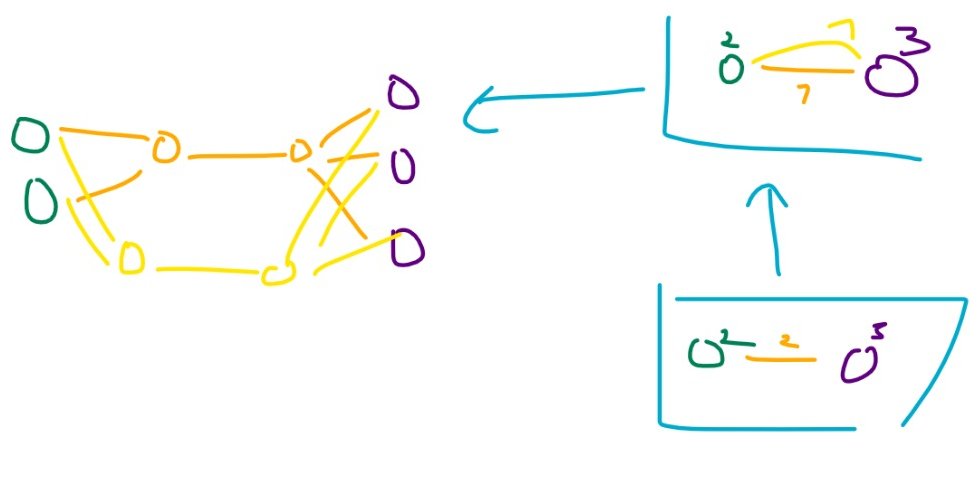
\includegraphics[width=.5\textwidth]{73graphs}
    \caption{Graph reduction}
    \label{fig:73graphs}
  \end{figure}

  When converting $X$ and $Y$ to this new graph $G'$ we treat them a little differently.
  Both sets include the $b(v)$ copies of all their vertices,
  but the vertices we added to each edge are only included in $Y'$ (not $X'$)
  and only when the connect to some other vertex outside of $X$ and $Y$.
  Even in this case $Y'$ only include half an edge, and the other paired vertex remains in $G' - X' - Y'$.

  With this arrangement the size of every connected component $C$ in $G' - X' - Y'$ will be
  $\sum_{c\in V(C)}b(c) + \sum_{e\in E_G(V(C),Y)}u(e)$.
  Additionally $G' - X' - Y'$ will have an even connected component of size $2$ for every edge inside $X$ and between $X$ and $Y$.
  This matches with what we need for Tutte's Theorem.

  The size of $|X' \dot\cup Y'|$ can also be calculated:
  \[ \sum_{v\in X}b(v) +
    \sum_{y\in Y}b(y) +
    \sum_{y\in Y}\sum_{e\in\delta(y)}u(e) -
    \sum_{e\in E_{G}(X,Y)}u(e) \]
  Which is almost what we need, except for the fact that the term $\sum_{y\in Y}b(y)$ is included with a plus, and not a minus...

  \subsection{Minimum weight $T^*$-joins}
  \begin{centerframebox}
    Let $G$ be an undirected graph and $T \subseteq V(G)$ such that $|T|$ is even.
    Show that the convex hull of incidence vectors of $T$-joins in $G$ is given by the set
    $P$ of all $x \in [0, 1]^{E(G)}$ satisfying
    \[ \sum_{e\in F}(1-x_{e}) + \sum_{e\in \delta(X) \setminus F} x_{e} \geq 1 \qquad
       \forall X\subseteq V(G),\, F\subseteq\delta(X)
       \textrm{ such that } |X\cap T|+|F| \textrm{ is odd }
    \]

    Hint: First show that the incidence vector of every $T$-join in $G$ satisfies the given
    constraints. Next, show that every vertex of $P$ is the incidence vector of a $T$-join
    in $G$ by showing that for each cost function $c \in \R^{E(G)}$, there exists a $T$-join $J$
    such that the incidence vector $\chi^J$ of $J$ minimizes $c^T x$ over $P$.
    To this end, let $E^{-} := \{e\in E(G):c(e)<0\}$ and, for a vector $x \in P$, consider the vector $\bar{x}$ given
    by

    \[
      \bar{x}_{e} =
      \begin{cases}
        x_{e} &, e \in E(G) \setminus E^{-} \\
        1-x_{e} &, e \in E^{-}
      \end{cases}
    \]

    and prove that $\bar{x}$ is contained in the up-hull of the $T \Delta \operatorname{odd}(E^-)$-polyhedron of $G$.
  \end{centerframebox}
  Let $x$ be an incidence vector of a T-join. Suppose $x$ satisfies not the given condition, then let $X\subseteq V(G), F\subseteq \delta(X)$ with $|X\cap T|+|F|$ odd such that $\sum_{e\in F}(1-x_{e}) + \sum_{e\in \delta(X) \setminus F} x_{e} < 1$. As $x$ is an incidence vector its entries  are $0$ or $1$, thus $\sum_{e\in F}(1-x_{e}) + \sum_{e\in \delta(X) \setminus F} x_{e} =0$, so $\forall e\in F: x_e=1$ and $ \forall e\in \delta(X) \setminus F: x_e=0$.
  If $|F|$ is odd, then as $x_e$ is a incidence vector of a T-join, $|X\cap T|$ is odd, which is a contradiction to $|X\cap T|+|F|$ odd. If $|F|$ is even, then as $x_e$ is a incidence vector of a T-join, $|X\cap T|$ is even, which is a contradiction to $|X\cap T|+|F|$ odd. Thus $x$  satisfies the given constraints.

  % TODO (Carola)

\end{document}
